\section{31. Oktober 2013}

\question{Bindungszustände / Elektronenkonfiguration in N2 diskutieren.}
\label{q:70}
Siehe \qref{52}.

\question{Skizzieren Sie die wesentlichen Elemente der Born-Oppenheimer Näherung.}
\label{q:71}

\question{Erklärung von Hybridisierung anhand sp, sp2 und sp3.}
\label{q:72}

\question{Lennard-Jones Potential und Van der Waals Bindung.}
\label{q:73}

Van der Waals Kräfte sind die relativ schwachen nicht weitreichende Wechselwirkungen zwischen Atomen oder Molekülen. Sie können ideale Gas Atome zusammenhalten, obwohl diese aufgrund ihrer neutralität keine Coulomb Anziehung zwischen sich haben.
Normalerweise ist das Dipolmoment eines solchen Atoms 0, jedoch kann durch Schwankungen der Ladung um ihre Durchschnittliche Position kurzzeitig eines entstehen. 
Das Nachbaratom reagiert auf dieses und es kommt zu einer anziehenden Kraft zwischen ihnen. Der Durchschnitt der Kräfte zwischen den Atomen ist die Van-der-Waals-Kraft. Diese Bindungen sind sehr schwach und die Bindungsenergie beträgt nur wenige meV.
Das Van-der-Waals Bindungspotential ist oft durch das Lennard-Jones-Potential angenähert. Dieses beschreibt in der Atom- und Molekülphysik die Bindungsenergie. Es nähert die Wechselwirkung zwischen ungeladenen, nicht chemisch aneinander gebundenen Atomen an.

\begin{align}
    U(R) = 4\epsilon[(\frac{\sigma}{R})^{12} - (\frac{\sigma}{R})^6]
\end{align}

Dabei entspricht $\epsilon$ der Tiefe der Potentialmulde, $\sigma$ dem Teilchenabstand an der Nullstelle und $R$ dem variierendem Abstand der Teilchen.\\

\begin{figure}[H]
    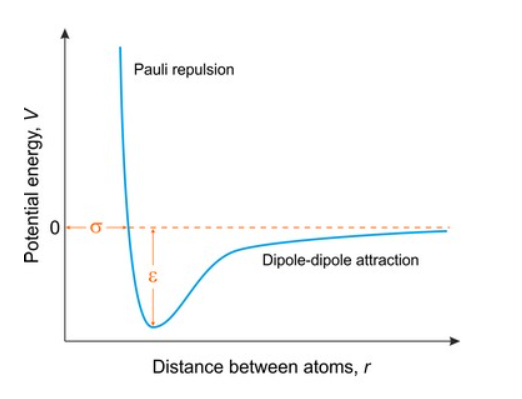
\includegraphics[width=0.8\linewidth]{resources/31-10-2013/lennard.PNG}
    \caption{Beispielhafter Plot des Lennard-Jones-Potentials}
\end{figure}

\question{Diskutieren Sie die Laue'sche Beugungsbedingung.\
\label{q:74}
\qquad \qquad a) Anhand der Ewald-Konstruktion.\
\qquad \qquad b) Im Rahmen der Bragg'schen Interpretation.}

\question{Skizzieren Sie die 1. Brillouin-Zone eines ebenen hexagonalen Gitters.}
\label{q:75}

\question{Gitterenergie in einem Ionenkristall.}
\label{q:76}

\question{Röntgenbeugung mit der Drehkristallmethode.}
\label{q:77}

\question{Vergleichen Sie das Einstein- und Debye-Modell der spezifischen Wärme. Welche Annahme ist in BEIDEN Modellen zu einfach?}
\label{q:78}

\newpage
\section{Juli 2017}

\question{Zeichne das Potential eines homöopolaren Moleküls. Beschreiben Sie es qualitativ.}
\label{q:79}

\question{Was bewirkt die Austauschenergie beim H2 Molekül? Wann ist sie groß/klein? Wieso ist sie für die chemische Bindung wichtig?}
\label{q:80}

Siehe \aqref{1}.

\question{Was kann man aus dem Rotations-Schwingungsspektrum für molekulare Größen bestimmen?}
\label{q:81}

Siehe \aqref{2}.

\question{Diskutieren Sie elektrische Rotations-Schwingungsübergänge und die Entstehung von Schwingungsbanden.}
\label{q:82}

Siehe \aqref{3}.

\question{Wie kann experimentell die Dispersionsrelationskurve von Phononen ermittelt werden?}
\label{q:83}

\question{Diskutieren Sie die Wärmekapazität sowohl in der klassischen als auch in der quantenmechanischen Betrachtung.}
\label{q:84}

\question{Was für ein Zusammenhang besteht zwischen der Gitterebene und einem Vektor im reziproken Raum?}
\label{q:85}

Siehe \aqref{4}.

\question{Erklären Sie das Auftreten von Energiebandlücken mit Hilfe des Models der fast freien Elektronen.}
\label{q:86}

siehe \aqref{5}

\question{Beschreiben Sie das Bloch-Theorem eines Elektrons im harmonischen Potential.}
\label{q:87}

\question{Diskutieren Sie die Zustandsdichte in Schwingungsspektren von Festkörpern.}
\label{q:88}